\chapter{Passive Optical Components}
Les composantes passifs ne convertissent pas l'énergie (pas d'émission, amplification ou 
conversion).

\section{Optical couplers}
	\begin{wrapfigure}[6]{l}{5.6cm}
	\vspace{-5mm}
	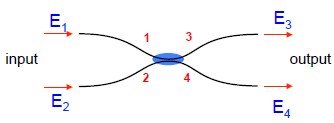
\includegraphics[scale=0.6]{ch3/image1}
	\captionof{figure}{ }
	\end{wrapfigure}
Le rôle d'un coupleur est de mélanger le signal venant de deux entrées différentes et diviser le 
signal mixé entre les différents ports de sortie. On peut alors combiner ou séparer des longueurs
d'ondes différentes (ce que font les\textit{ wavelength division multiplexing systems} (WDM/DWDM
 couplers)). Le plus simple est le coupleur $2\times2$ que l'on peut voir comme une version 
 fibrée/intégrée d'un semi-miroir de transmission $\epsilon^2$. La matrice (s'il est sans perte) est
 d'ailleurs similaire à celle d'un semi-miroir
\begin{equation}
\left( {\begin{array}{*{20}{c}}
{{E_3}}\\
{{E_4}}
\end{array}} \right) = \left( {\begin{array}{*{20}{c}}
\varepsilon &{j\sqrt {1 - {\varepsilon ^2}} }\\
{j\sqrt {1 - {\varepsilon ^2}} }&\varepsilon 
\end{array}} \right)\left( {\begin{array}{*{20}{c}}
{{E_1}}\\
{{E_2}}
\end{array}} \right)
\end{equation}
où $\epsilon^2$ est la fraction d'énergie $1\to 4$ ou $2\to 3$ et la partie complexe découle de la
conservation d'énergie.


\subsection{Physical principle and analytical model}
	\begin{wrapfigure}[6]{r}{7cm}
	\vspace{-5mm}
	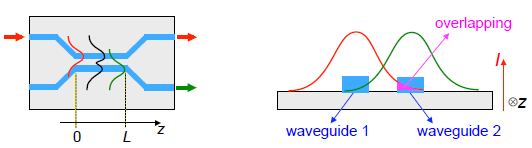
\includegraphics[scale=0.5]{ch3/image2}
	\captionof{figure}{ }
	\end{wrapfigure}
On va utiliser les propriétés des fibres pour essayer de coupler de l'énergie de l'une à l'autre. 
Si on place des fibre suffisamment proche, les modes évanescents vont se couvrir et il y aura
échange d'énergie entre les deux guides d'ondes avec la distance de propagation. \\

Si ce recouvrement n'induit qu'une "perturbation" (pas de grosse modification du profil du mode et
de sa constante de propagation), l'évolution des amplitudes de $\vec{E}$ est donnée par un système de 
deux équations couplées. 
\begin{equation}
\left\{\begin{array}{ll}
\dfrac{{d{A_1}}}{{dz}} &\DS=  - j{C_{12}}{e^{ - j\Delta \beta z}}{A_2}\vspace{2mm}\\
\dfrac{{d{A_2}}}{{dz}} &\DS=  - j{C_{21}}{e^{j\Delta \beta z}}{A_1}
\end{array}\right.
\end{equation}
où $C_{ij}$ est la constante de couplage, qui augmente avec le recouvrement des modes et 
où $\Delta\beta = \beta_2-\beta_1$, la différence entre les constantes de propagation.\\

	\begin{wrapfigure}[6]{r}{4.5cm}
	\vspace{-10mm}
	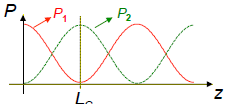
\includegraphics[scale=0.75]{ch3/image3}
	\captionof{figure}{ }
	\end{wrapfigure}
Ici, on regarde ce qui se passe \textit{dans} le coupleur alors que la précédente matrice ne liait que l'entrée à la sortie. Supposons que les deux guides d'ondes soient identiques $\Delta\beta=0,
C_{12}=C_{21}=C_0$.  En prenant comme C.I. $A_1(0) = \sqrt{P_0}$ et $A_2(0)=0$, on trouve une 
solution en cosinus pour $P_1$ et en sinus pour $P_2$
\begin{equation}
{P_1}(z) = {A_1}{^2} = {P_0}{\cos ^2}({C_0}z)\qquad\qquad\qquad
{P_2}(z) = {A_2}{^2} = {P_0}{\sin ^2}({C_0}z)
\end{equation}
On observe une variation périodique de l'énergie dans chaque guide d'onde. Le signal n'est inséré 
que dans un seul guide d'onde et toute l'énergie est transférée dans le second en 
$z=(2m+1)L_c$ où $L_c=\pi/(2C_0)$ est la longueur de couplage. On voit donc que plus le couplage
est fort, plus il sera rapide en terme de distance. Notons que $L_c = f(\lambda)$. Des exemples de
coupleurs sont donnés au \textit{slide 6}.\\


	\begin{wrapfigure}[11]{l}{10.5cm}
	\vspace{-5mm}
	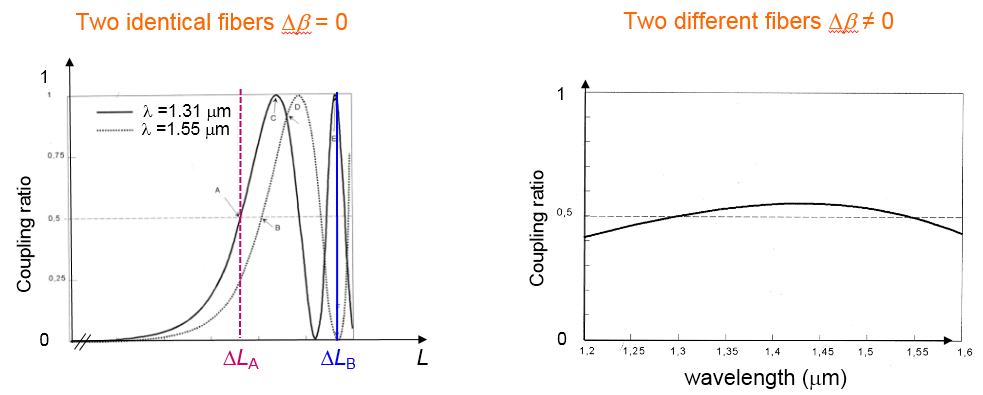
\includegraphics[scale=0.4]{ch3/image4}
	\captionof{figure}{ }
	\end{wrapfigure}
Intéressons-nous à l'évolution du rapport de couplage en fonction de l'étirement $L$. Soit le cas
de deux fibres identiques, $\Delta\beta=0$. Si on l'étire jusqu'au point $\Delta L_A$ on obtient un
coupleur 50/50 chromatique, à une longueur d'onde donnée. Ce qui est intéressant, c'est l'étirement
jusqu'à $\Delta L_B$. Il s'agit de la solution ou l'on obtient un maximum de couplage pour 1.3 $\mu$m
et un minimum pour $1.5\mu$m : c'est le WDM, qui va permettre de séparer les deux.\\
 
Supposons que l'on ai deux sortie, $P_3$ et $P_4$. Le graphique nous donne $P_4/(P_4+P_3)$. Quand
celui-ci vaut 1, tout sort part $P_4$ et quand il vaut 0, par $P_3$. Si on envoie donc un mélange
des deux longueurs d'onde dans une entrée d'un coupleur où $L=\Delta L_B$, $\lambda=1.5\mu$m va
sortie en $P_3$ et $\lambda=1.3\mu$m va sortie en $P_4$. On peut également prendre des fibres 
différentes ($\Delta\beta\neq0$) mais le ration de couplage maximum sera inférieur à 100\%.\\

Il existe également des coupleurs en étoile ($N\times N$ ou $N\times M$) qui \textbf{combinent} 
les signaux des $N$ entrées et les divise \textit{équitablement} entre les $N$ ($M$) sorties. C'est
typiquement le cas des réseaux LAN. Deux exemples sont donnés \textit{slide 8}. Notons qu'avec de
tel système, on ne peut pas séparer les polarisations.



\section{Polarization controllers (PC)}
Le SOP d'une fibre est à priori inconnu et peut changer. Parfois, il est nécessaire de contrôler
celui-ci (composants sensibles à la polarisation, systèmes de multiplexage, systèmes de 
polarisation cohérentes, \dots). \\

Un contrôleur de polarisation (PC) peut transformer n'importe quel SOP d'entrée en un SOP de 
sortie voulu (soit n'importe où sur la sphère de Poincaré). Évidemment, il faudra des systèmes
dynamiques pour les télécommunications. Il existe deux principes physiques
\begin{description}
\item[Cristal biréfringent] utiliser des lames à retard. Le problème c'est qu'il faut sortir du
guide, passer le cristal et revenir dans le guide : pertes. De plus, l'inertie des lames limite 
la vitesse de changement.
\item[Contraintes] modifie la biréfringence de la fibre en la bouclant, pressant, tordant, \dots
Peu de pertes par insertion, pas de back-reflection et rapide ($\approx30\ \mu$s).
\end{description}

	\begin{wrapfigure}[11]{l}{9cm}
	\vspace{-5mm}
	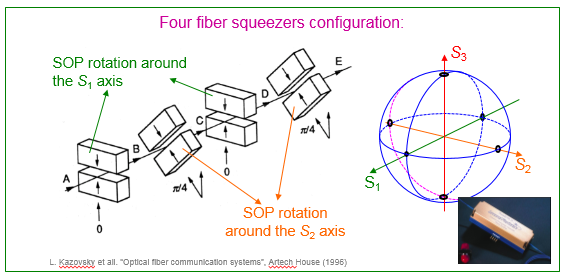
\includegraphics[scale=0.6]{ch3/image5}
	\captionof{figure}{ }
	\end{wrapfigure}
La meilleure technique actuelle est d'utiliser un feedback automatique pour contrôler les contraintes
appliquées à la fibre, à l'aide de quatre "compresseurs" piézoélectriques. En fixant les compresseurs
on fixe les axes de biréfringence et en modifiant la force qu'ils appliquent on modifie le saut
de phase. L'avantage est qu'il est insensible à la longueur d'onde et qu'il n'y a pas d'effet de
reset. 


\section{Isolateurs et circulateurs}
Un isolateur autorise la transmission dans une direction, mais la bloque dans toutes les autres. Il
s'agit d'un composant \textbf{non}-réciproque, celle-ci venant de l'effet Faraday intervenant
lorsqu'un champ d'induction magnétique $\vec{B}$ longitudinal est appliqué au milieu. En présence
d'un champ d'induction magnétique $\vec{f} = -q\vec{B}\times\vec{v}$.\\

Pour un dipôle circulaire 
en rotation trigonométrique, cette force pointera vers le centre de rotation et inversement pour
un dipôle. Cette force va ainsi causer la rotation d'un SOP linéaire d'un angle $\beta$. Lorsque
de la lumière sera réfléchie, la polarisation va se "retourner" et la force appliquée sera dans
le même sens : le sens de rotation est identique dans les deux direction, c'est l'effet 
non-réciproque. 
\begin{center}
	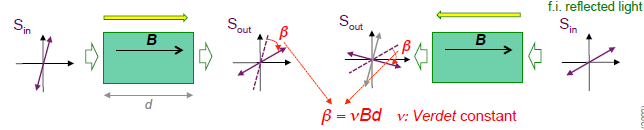
\includegraphics[scale=0.76]{ch3/image6}
	\captionof{figure}{Rotation des SOP linéaires d'un angle $\beta = \nu Bd$ où $\nu$ est la
	constante de Verdet, $B$ la norme du champ d'induction magnétique et $d$ la distance de 
	propagation. Le sens de rotation est indépendant du sens de propagation.}
\end{center}
Généralement, on met un polariseur de sorte à ne laisser passer la lumière qui revient qu'à cette
polarisation-là. On travaille ainsi avec $\beta=45^\circ$ tel que la lumière réfléchie est polarisée 
orthogonalement par rapport à la lumière à l'entrée de l'isolateur. Cependant, dans une fibre ce
n'est pas pratique : on veut quelque chose d'insensible à la polarisation (fortes variation dans une fibre). 

\begin{center}
	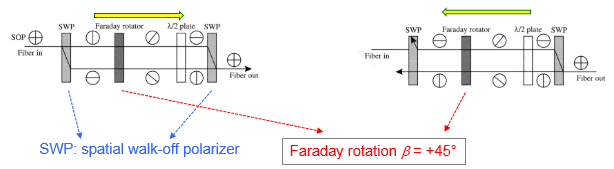
\includegraphics[scale=0.76]{ch3/image7}
	\captionof{figure}{ }
\end{center}

Pour les isolateurs insensibles à la polarisation, on va d'abord séparer le faisceau en deux à 
l'aide d'un cristal biréfringent (SWP) tel que la polarisation horizontale et verticale soient
séparées spatialement mais parallèles. On les fait ensuite passer dans le rotateur puis par une
lame $\lambda/2$ avant de les "recombiner" dans un second SWP. Si de la lumière vient de l'autre
sens, après le rotateur elle aura une direction qui n'est pas celle du cœur : angle trop important,
rien ne sera excité et toute l'énergie sera radiée (cf. flèche dans SWP)\footnote{A ré-expliquer}. 
Le \textit{slide 13} donne un exemple. Remarquons les faibles pertes par insertion (0.6 dB) malgré 
tout ce qui se trouve dans un tel dispositif. \\

	\begin{wrapfigure}[4]{r}{2cm}
	\vspace{-10mm}
	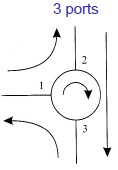
\includegraphics[scale=0.6]{ch3/image8}
	\captionof{figure}{ }
	\end{wrapfigure}
Il existe aussi des circulateurs : le fonctionnement est le même que pour des isolateurs mais
il y a plus que deux ports (même principes (non-réciproque) mais géométrie plus subtile). Ci-contre,
la lumière qui rentre dans 1 peut aller dans 2 mais celle de 2 ne peut pas aller dans 1, mais 
seulement 3 etc.



\section{Fiber Bragg gratings}

	\begin{wrapfigure}[9]{l}{6.5cm}
%	\vspace{-5mm}
	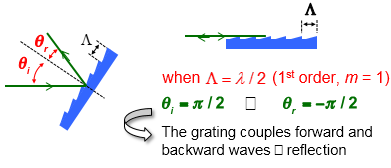
\includegraphics[scale=0.6]{ch3/image9}
	\captionof{figure}{ }
	\end{wrapfigure}
Les réseaux de Bragg fibrés se basent sur l'équation des réseaux\footnote{Variation périodique de 
$n$.}
\begin{equation}
\sin ({\theta _i}) - \sin ({\theta _r}) = m\frac{\lambda }{\Lambda }
\end{equation}
où $m$ est l'ordre de diffraction et $\Lambda$ la période de modulation spatiale. 
Lorsque $\Lambda=\lambda/2$ (au premier ordre), $\theta_i=\pi/2\ \to\ \theta_r = -\pi/2$ : le 
réseau couple l'onde back et forward, soit de la \textbf{réflexion}.\\

	\begin{wrapfigure}[6]{r}{6.5cm}
	\vspace{-5mm}
	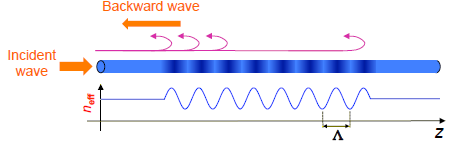
\includegraphics[scale=0.6]{ch3/image10}
	\captionof{figure}{ }
	\end{wrapfigure}
A cause de la variation d'indice de réfraction, l'énergie du mode back et couplée à celle du mode
forward pour les longueur d'ondes proche de la longueur d'onde de Bragg $\lambda_B = 2n_{eff}\Lambda$
où $\Lambda$ est la période du réseau et $n_{eff}$ l'indice effectif du mode guidé. \\

Comme les coefficients sont très dépendant de $\lambda$, il est possible d'en faire des filtres
en réflexion.




\newpage
\subsection{Propagation dans un réseau de Bragg fibré (théorie des modes couplés)}
Faisons quatre  hypothèses
\begin{enumerate}
\item SMF, $E(x)$ (polarisation linéaire)
\item Période de la constante diélectrique constante dans la direction $z$
\item Le profil transverse du mode $U(x,y)$ est constant (pas affecté par la modulation d'indice)
\item La SVEA s'applique
\end{enumerate}
On peut alors écrire le champ électrique sous la forme
\begin{equation}
E\left( {x,y,z,t} \right) = {{\bf{1}}_x}A(z)U(x,y)\exp \left( {j{\omega _0}t} \right)
\end{equation}
Et l'équation de propagation
\begin{equation}
\Delta {\tilde  E + }\kappa (x,y,z)\frac{{\omega _0^2}}{{{c^2}}}\tilde E = 0
\end{equation}
Considérons une variation périodique de $\kappa$, la constante diélectrique, comme sa série de
Fourier au premier ordre (équivalent à considérer uniquement le premier ordre de diffraction 
du réseau)
\begin{equation}
\kappa {\kappa _0}(x,y) + \underbrace{\Delta \kappa (x,y)\cos (2\pi z/\Lambda )}_{\Delta \kappa}
\end{equation}
où $\Delta\kappa(x,y)\ll 1$ (modes imperturbés). Il s'agit donc du saut d'indice permettant la 
modulation et d'une petite modulation (pouvant être $f(x,y)$) cosinusoïdale. \\

Dans le réseau, pour $\lambda\approx\lambda_B$, il y a un couplage entre l'onde for ($A_F$) 
et backward ($A_B$). La solution est une superposition entre ces deux ondes contra-propagatives
\begin{equation}
A(z) = {A_F}(z){e^{ - j{\beta _0}z}} + {A_B}(z){e^{ + j{\beta _0}z}}
\end{equation}
Il suffit de tout injecter. Le champ étant transverse, on va séparer la partie transverse du 
Laplacien. La dérivée seconde de l'amplitude en $z$ donne
\begin{equation}
\frac{{{{\rm{d}}^2}A}}{{{\rm{d}}{z^2}}} =  - \beta _0^2A + \left( { - 2j{\beta _0}\frac{{{\rm{d}}{A_F}}}{{{\rm{d}}z}}{e^{ - j{\beta _0}z}} + 2j{\beta _0}\frac{{{\rm{d}}{A_B}}}{{{\rm{d}}z}}{e^{ + j{\beta _0}z}}} \right) + \left( {\frac{{{{\rm{d}}^2}{A_F}}}{{{\rm{d}}{z^2}}}{e^{ - j{\beta _0}z}} + \frac{{{{\rm{d}}^2}{A_B}}}{{{\rm{d}}{z^2}}}{e^{ + j{\beta _0}z}}} \right)
\end{equation}
où la deuxième parenthèse s'annule (SVEA). En remplaçant ce résultat dans l'équation de propagation
\begin{equation}
\beta _0^2AU + U\left( { - 2j{\beta _0}\frac{{{\rm{d}}{A_F}}}{{{\rm{d}}z}}{e^{ - j{\beta _0}z}} + 2j{\beta _0}\frac{{{\rm{d}}{A_B}}}{{{\rm{d}}z}}{e^{ + j{\beta _0}z}}} \right) + A{\Delta _ \bot }U + ({\kappa _0} + \delta \kappa )\frac{{\omega _0^2}}{{{c^2}}}AU = 0
\end{equation}
où $\Delta_T$ est le Laplacien transverse. Rappelons que la séparation des variables 
$E=A(z)U(x,y)$ peut se faire car $n(z)$ ne modifie pas le profil transverse du mode $U(x,y)$.
En reconnaissant l'équation modale ${\Delta _ \bot }U + ({\kappa _0}\frac{{\omega _0^2}}{{{c^2}}} -
 \beta _0^2)U = 0$, l'équation de propagation devient
 \begin{equation}
 \left( { - 2j{\beta _0}\frac{{{\rm{d}}{A_F}}}{{{\rm{d}}z}}{e^{ - j{\beta _0}z}} + 2j{\beta _0}\frac{{{\rm{d}}{A_B}}}{{{\rm{d}}z}}{e^{ + j{\beta _0}z}}} \right)U + \frac{{\Delta \kappa }}{2}\left( {{e^{ + \frac{{j2\pi z}}{\Lambda }}} + {e^{ - \frac{{j2\pi z}}{\Lambda }}}} \right)\left( {{A_F}{e^{ - j{\beta _0}z}} + {A_B}{e^{ + j{\beta _0}z}}} \right)\frac{{\omega _0^2}}{{{c^2}}}U = 0
 \end{equation}
où $\delta\kappa$ a été écrit en exponentielle pour simplifier le problème. \\

En multipliant l'équation par le conjugué du profil transverse $U*$ et en intégrant sur tout le
profil transverse\footnote{\danger\ $\delta k$ peut dépendre de $x$ et $y$, on ne peut pas le sortir
de l'intégrale.} $\int\dots \times U*\ dx\ dy$ 
\begin{equation}
\left( { - j\frac{{{\rm{d}}{A_F}}}{{{\rm{d}}z}}{e^{ - j{\beta _0}z}} + j\frac{{{\rm{d}}{A_B}}}{{{\rm{d}}z}}{e^{ + j{\beta _0}z}}} \right) + C\left( {{e^{ + \frac{{j2\pi z}}{\Lambda }}} + {e^{ - \frac{{j2\pi z}}{\Lambda }}}} \right)\left( {{A_F}{e^{ - j{\beta _0}z}} + {A_B}{e^{ + j{\beta _0}z}}} \right) = 0
\end{equation}
où $C$ est le coefficient de couplage entre les mode back et forward défini par 
\begin{equation}
C = \frac{1}{{4{\beta _0}}}\frac{{\omega _0^2}}{{{c^2}}}\frac{{\int {\Delta \kappa (x,y)|U{|^2}{\rm{d}}x{\rm{d}}y} }}{{\int {|U{|^2}{\rm{d}}x{\rm{d}}y} }}
\end{equation}
avec ${\int {\Delta \kappa (x,y)|U{|^2}{\rm{d}}x{\rm{d}}y} }$ l'intégrale d'overlap entre la 
modulation de l'indice et le profil modal.\\

Pour la suite, il est plus simple d'écrire l'ED sous la forme de deux ED couplée. On va faire une
sorte "d'intégrale glissante" sur un petit $\delta z$, une sorte de moyenne. On peut faire ça car
beaucoup de termes oscillants dont certains qui vont s'annuler en moyenne (celui de $A_B$ notamment).
En multipliant par $e^{+j\beta_0z}$, en prenant la moyenne sur $z$ et avec la SVEA, 
on trouve\footnote{Un terme oscillant sera à moyenne nulle. Par contre si $2\beta_0$ est proche de
$2\pi/\Lambda$, l'oscillation sera très lente et il faudra garder ce terme.}
\begin{equation}
\frac{{{\rm{d}}{A_F}}}{{{\rm{d}}z}} =  - jC{A_B}{e^{2j{\beta _0}z - 2j\frac{\pi }{\Lambda }z}} =  -
 jC{A_B}{e^{2j\delta z}}
\end{equation}
Le terme en $A_B$ tombe et le terme croisé (celui en $C(\dots)(\dots)$) correspond à la deuxième
contribution exponentielle. En faisant de même, mais en multipliant par $e^{-j\beta_0z}$ on trouve
\begin{equation}
\frac{{{\rm{d}}{A_B}}}{{{\rm{d}}z}} = jC{A_F}{e^{ - 2j\delta z}}
\end{equation}
où $\delta  = {\beta _0}({\omega _0}) - \frac{\pi }{\Lambda }$.\\


	\begin{wrapfigure}[2]{r}{5cm}
	\vspace{-8mm}
	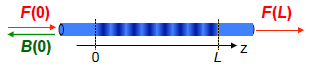
\includegraphics[scale=0.6]{ch3/image11}
	\captionof{figure}{ }
	\end{wrapfigure}
Posons ${A_F} = F{e^{ + j\delta z}}\;$ et ${A_B} = B{e^{ - j\delta z}}$. On en tire un système 
de deux équations différentielles linéaires couplées
\begin{equation}
\left\{\begin{array}{ll}
\dfrac{{{\rm{d}}F}}{{{\rm{d}}z}} &\DS=  - j\delta F - jCB\vspace{2mm}\\
\dfrac{{{\rm{d}}B}}{{{\rm{d}}z}} &\DS=  + j\delta B + jCF
\end{array}\right.
\end{equation}
Considérons comme CL que l'on injecte de la lumière d'un côté ($F(0)=F_0$) mais pas de l'autre 
$(B(L)=0)$. Soit le \textbf{detuning parameter}, crucial
\begin{equation}
\delta  = {\beta _0}({\omega _0}) - \frac{\pi }{\Lambda }
\end{equation}
elui-ci "mesure" à quelle distance on se situe de la condition de réflexion de Bragg à travers la différence entre la constante de propagation du mode et le nombre d'onde du réseau $\pi/\Lambda$.\\

Pour déterminer le coefficient de réflexion de Bragg $B(0)/F(0)$, il faut donc résoudre les deux
équations couplées avec les CL. Ceci se fait en calculant les vecteurs propres de la matrice, pour
trouver
\begin{equation}
\left( {\begin{array}{*{20}{c}}
F\\
B
\end{array}} \right) = {A_1}\left( {\begin{array}{*{20}{c}}
{\delta  - j\zeta }\\
{ - \;C}
\end{array}} \right)\exp ( - \zeta z) + {A_2}\left( {\begin{array}{*{20}{c}}
{\delta  + j\zeta }\\
{ - \;C}
\end{array}} \right)\exp ( + \zeta z)
\end{equation}
où $\xi = \sqrt{C^2-\delta^2}$. On en tire que
\begin{equation}
\rho (\omega ) = \frac{{B(0)}}{{F(0)}} = \frac{{ - C\sinh (\zeta L)}}{{\delta \sinh (\zeta L) - j\zeta \cosh (\zeta L)}}
\end{equation}
La \textbf{réflectance} vaut alors
\begin{equation}
R = \rho \;{^2} = \frac{{{{\sinh }^2}(\zeta L)}}{{{{\cosh }^2}(\zeta L) - {\delta ^2}/{C^2}}}
\end{equation}
Si la longueur d'onde réfléchie est telle que $\delta < C$, alors $\xi$ est réel : ces longueurs
d'ondes subissent une décroissance exponentielle et ne se propagent pas et toute l'énergie est
transférée au \textbf{mode backward}.\\

Intéressons-nous à comment varie $R$ et l'augmentation de la bande passante avec le coefficient de 
couplage $C$ et la longueur $L$ du réseau. Lorsque le produit $CL$ est suffisamment grand, on peut
obtenir $R=1$ : tout le couplage à le "temps" de se faire. On voit une évolution de la phase 
non-linéaire (sinon on aurait des différence de vitesse de groupe et donc de la dispersion 
chromatique). Si le produit $CL$ est trop petit, on n'atteint pas la valeur maximale. Cela signifie
que le couplage entre back et forward est trop faible, c'est comme si on "coupait tôt" le couplage
et qu'une partie de l'énergie arrive au bout et s'échappe (transmission).

\begin{center}
	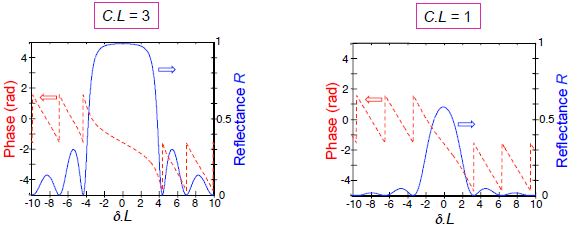
\includegraphics[scale=0.8]{ch3/image12}
	\captionof{figure}{ }
\end{center}

	\begin{wrapfigure}[7]{l}{4cm}
	\vspace{-8mm}
	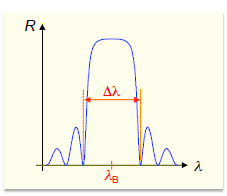
\includegraphics[scale=0.6]{ch3/image13}
	\captionof{figure}{ }
	\end{wrapfigure}
La bande passante en réflexion $\Delta\lambda$ dépend aussi de $L$ et $C$. Ce paramètre est
important car il permet de sélectionner un canal précis. Réécrivons le sinh en inversant $C$ et
$M$
\begin{equation}
\sinh (\zeta L) = 0 \Rightarrow \sin (\sqrt {{\delta ^2}{L^2} - {C^2}{L^2}} ) = 0
\end{equation}
Sachant que $\left| \delta  \right| = \sqrt {\frac{{{\pi ^2}}}{{{L^2}}} + {C^2}}  \approx 2\pi
 {n_{eff}}\frac{{\left| {{\lambda _B} - \lambda } \right|}}{{\lambda _B^2}}$, on en tire\\
 
 \cadre{\begin{equation}
 \frac{{\Delta \lambda }}{{{\lambda _B}}} = \frac{{{\lambda _B}}}{{\pi {n_{eff}}}}C\sqrt
  {{{(\frac{\pi }{{LC}})}^2} + 1} 
 \end{equation}}\ \\
 
 Il en découle deux cas de figure
 \begin{enumerate}
 \item "Faible" couplage ($CL\ll 1$)
 \begin{equation}
{\lambda _B} = 2{n_{eff}}\Lambda  \Rightarrow \frac{{\Delta \lambda }}{{{\lambda _B}}} =
 2\frac{\Lambda }{L}
 \end{equation}
 Plus le réseau est grand, plus $\Delta\lambda$ va être sélectif. Dans les spectromètre à réseau, 
 la résolution spectrale est liée au nombre de traits interceptés.
 \item "Fort" couplage ($CL \gg 1$)
 \begin{equation}
 \frac{{\Delta \lambda }}{{{\lambda _B}}} \to \frac{{{\lambda _B}C}}{{\pi {n_{eff}}}}
 \end{equation}
 Le bande-passante est indépendante de $L$ et proportionnelle à $C$, soit $\Delta \kappa$ soit
 $\Delta n$.
 \end{enumerate}

\begin{center}
	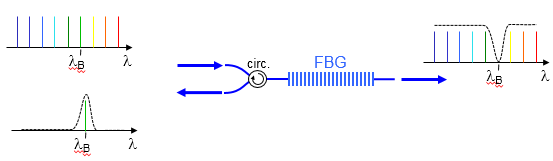
\includegraphics[scale=0.8]{ch3/image14}
	\captionof{figure}{La sélection se fait bien en réflexion, d'où l'utilité d'un circulateur
	pour faire un WDM avec un réseau de Bragg fibré. Lire remarques \textit{slide 24}.}
\end{center}


\subsection{Chirped Fiber gratings for GVD compensation}
	\begin{wrapfigure}[7]{l}{8.5cm}
	\vspace{-5mm}
	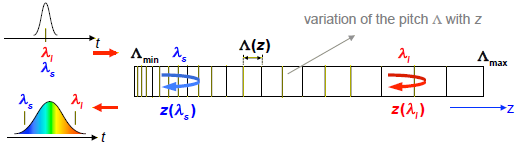
\includegraphics[scale=0.6]{ch3/image15}
	\captionof{figure}{ }
	\end{wrapfigure}
Un moyen de compenser la dispersion est d'utiliser des réseaux de Bragg fibré chirped\footnote{On 
va d'une période élevée vers une plus basse ici.} : le pas du réseau n'est pas constant et change 
sur sa longueur. Ceci implique que la longueur de Bragg varie avec $z$. Dès lors, la position de
la réflexion d'une longueur d'onde dépend de la longueur d'onde elle-même : le temps pour qu'un
paquet d'onde soit réfléchi est ainsi aussi dépendance de la longueur d'onde. Les variations dans
le rouge sont retardées par rapport à celle dans le bleu. L'idée est de faire l'inverse pour 
compenser la dispersion causée par un chirped linéaire.\\


	\begin{wrapfigure}[13]{r}{5.5cm}
	\vspace{-5mm}
	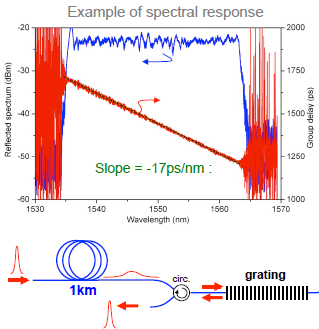
\includegraphics[scale=0.6]{ch3/image16}
	\captionof{figure}{ }
	\end{wrapfigure}
Calculons la "position" $z$ de réflexion d'une longueur d'onde particulière. Sachant que la longueur
d'onde réfléchie est donnée par $\lambda (z) = 2\Lambda (z){n_{eff}}$, on en tire
\begin{equation}
\frac{{\Delta \lambda }}{{\Delta z}} = 2{n_{eff}}\frac{{\Delta \Lambda }}{{\Delta z}}
\end{equation}
Le paramètre important est donc le gradient de pas du réseau. On peut également définir un temps
de vol (délai de groupe) correspondant au temps de vol entre l'entrée et la sortie d'un groupe
de fréquence. Celui-ci vaut la distance physique d'un aller/retour divisé par la vitesse de groupe
moyenne $v_g$
\begin{equation}
{\tau _g}(\lambda ) = 2z(\lambda )/{v_g}
\end{equation}
Le délai de groupe différentiel est donné par $\Delta \tau  = 2\Delta z/{v_g}$. Sachant que
\begin{equation}
\frac{{\Delta \lambda }}{{\Delta \tau (\lambda )}} = \frac{{\Delta \lambda }}{{\Delta z}}\frac{{{v_g}}}{2} = \frac{{\Delta \Lambda }}{{\Delta z}}\frac{{{v_g}}}{2}2{n_{eff}} = \frac{{\Delta \Lambda }}{{\Delta z}}{v_g}{n_{eff}}
\end{equation}
On en tire 
\begin{equation}
\frac{{\Delta \tau }}{{\Delta \lambda }} = {\left( {{v_g}{n_{eff}}\frac{{\Delta \Lambda }}{{\Delta z}}} \right)^{ - 1}}
\end{equation}
Ceci nous donne le décalage temporel $\Delta \tau$ accumulé par deux longueur d'ondes séparées de
$\Delta \lambda$. On voit que la dispersion de la vitesse de groupe est inversement proportionnelle
au gradient du pas du réseau. 


\subsection{Simple model of the linearly chirped grating: Transfer function in reflection}
On s'en doute un peu : le rôle du réseau de Bragg chirped, c'est de modifier la phase spectrale. 
Dans le domaine spectral, la fonction de transfert est donnée par
\begin{equation}
{\tilde A_{out}}(\omega ) = \tilde H(\omega ){\tilde A_{in}}(\omega )
\end{equation}
où $\tilde H(\omega ) = \tilde H(\omega )\;{{\mathop{\rm e}\nolimits} ^{j\tilde \varphi (\omega )}}$
avec $|\tilde{H}|$ l'amplitude (limitation de la BP) et $\tilde{\varphi}$ la phase (group delay
dispersion). Le délai de groupe est relié à la phase spectrale par ${\tau _g} =  - \frac{{\partial
\tilde \varphi }}{{\partial \omega }}$. En dérivant par rapport à $\lambda$
\begin{equation}
\frac{{\partial {\tau _g}}}{{\partial \lambda }} = {\left( {{v_g}{n_{eff}}\frac{{\Delta \Lambda }}{{\Delta z}}} \right)^{ - 1}} =  - \frac{\partial }{{\partial \lambda }}\frac{{\partial \tilde \varphi }}{{\partial \omega }} = \frac{{2\pi c}}{{{\lambda ^2}}}\frac{{{\partial ^2}\tilde \varphi }}{{\partial {\omega ^2}}} = \frac{{2\pi c}}{{{\lambda ^2}}}2a
\end{equation}
où on a utilisé $\frac{d}{d\lambda} = \frac{2\pi c}{\lambda^2}\frac{d}{d\omega}$ puis considéré
que $2\pi c/\lambda^2$ est constant de sorte à poser une autre constante $2a$ valant
\begin{equation}
{\left. {\frac{{{\partial ^2}\tilde \varphi }}{{\partial {\omega ^2}}}} \right|_{{\omega _0}}} = 2a\;
\; \Rightarrow \;\;\tilde \varphi  = a{(\omega  - {\omega _0})^2} - {\tau _p}(\omega  - {\omega _0})
 + {\tilde \varphi _0}
\end{equation}


La dérivée première de la phase spectrale est le délai moyen de toute l'impulsion lorsqu'elle 
fait un A/R dans le réseau de Bragg chirped, on le note $\tau_p$. On peut également avoir un terme
de phase constante du à la propagation. On remarque également une phase quadratique induite par le
réseau chirped, qui est le paramètre important ici (servira à compenser la phase quadratique induite
par la dispersion)
\begin{equation}
\tilde H(\omega ) = \tilde H(\omega )\;\exp [ja{(\omega  - {\omega _0})^2}]\exp [j{\tau _p}(\omega  -
 {\omega _0}) + j{\tilde \varphi _0}]
\end{equation}

\subsection{Bandwidth limitations}
Hélas, on ne peut pas faire ce que l'on veut : il va y avoir un impact sur la bande passante. En
effet, la bande passante du réseau ($\Delta\lambda$) et la dispersion induite par le réseau ($D_g$)
ne sont pas indépendantes à cause de la longueur finie du réseau $L_g$. Soit $D_g$, le paramètre 
de dispersion du réseau. Par définition
\begin{equation}
\frac{{\Delta {\tau _g}}}{{\Delta \lambda }} = \frac{{2\pi c}}{{{\lambda ^2}}}.2a \buildrel \Delta
\over = {L_g}.{D_g}
\end{equation}
Le temps de vol est donné par $\Delta {\tau _g} = {\tau _g}({\lambda _{\min }}) - {\tau _g}({\lambda
_{\max }}) = \frac{{2{L_g}}}{{{v_g}}} = {L_g}{D_g}\Delta \lambda$. On "peut" écrire ce genre de
relation car on se trouve dans le cas d'une variation quadratique de la phase. Dès lors\\

\cadre{\begin{equation}
{D_g} = \frac{{2{n_{eff}}}}{{c\Delta \lambda }}
\end{equation}
Une grande bande-passante implique un $D_g$ petit, il faudra faire un compromis entre BP importante
ou dispersion importante.}\ \\

\exemple{\textit{Soit $\Delta\lambda = 0.2$ nm $\to\ D_g = 5\times 10^7$ ps/km/mm ($n_{eff}
\approx1.5$). Si $L=10$ cm, ce réseau peut compesner la propagation sur \dots\ km d'une fibre
standard à $1.5\mu$m}.\\

On peut réutiliser la précédente relation
\begin{equation}
\sum_j L_jD_j = 0\qquad\Leftrightarrow\qquad L_FD_F = L_gD_g \qquad\Leftrightarrow\qquad
L_F = 333\ \text{km}
\end{equation}
La longueur de compensation est très importante, mais on sélectionne ici un seul canal. Il faut plus
de fibre à compensation de dispersion que $10$ cm, mais avec elle on compense toute la bande $C$.}


\section{(Tunable) Optical Filters}

	\begin{wrapfigure}[8]{r}{4cm}
	\vspace{-5mm}
	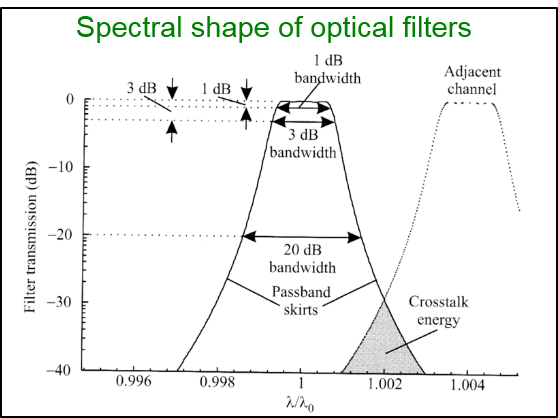
\includegraphics[scale=0.3]{ch3/image17}
	\captionof{figure}{ }
	\end{wrapfigure}
Les filtres passe-bande sont des composants très importants, par exemple avant un détecteur, pour 
les WDM, pour supprimer le bruit des amplificateurs optiques, \dots\ Un bon filtre doit avoir des
IL faible, une faible dépendance en la température, une bande passante plate afin d'éviter les 
distorsion de l'amplitude spectrale et des extensions raides pour éviter les \textit{crosstalk}
entre les canaux adjacent (un flanc vertical n'est pas réalisable en pratique). 

\subsection{The Fabry-Perot filter}
Il filtre FP est constitué d'une cavité linéaire construite avec deux miroirs semi-transparents 
de coefficient de réflexion en intensité $R$, supposé ici sans pertes. Pour certaines fréquences,
il va y avoir l'accumulation d'une phase multiple de $2\pi$ : résonance. Ces résonances auront 
lieux lorsque $2d=m\lambda$ où $m$ est entier. L'onde incidente et réfléchie interagiront de
façon constructive et la transmission est alors maximale.

\begin{center}
	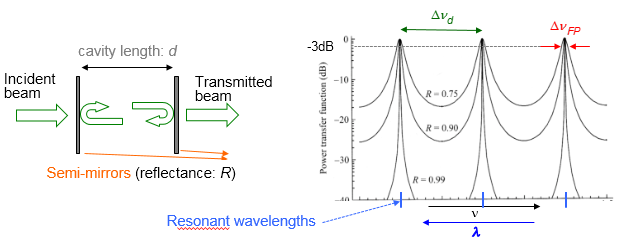
\includegraphics[scale=0.75]{ch3/image18}
	\captionof{figure}{ }
\end{center}

Définissons le \textit{Free Spectral Range} (FSR) $\Delta\nu_d$ comme l'écart spectral entre deux
pics de résonances. Plus $R\to1$, meilleur sera la sélectivité spectrale (qui vaudra cependant
toujours l'unité à la résonance, pour autant qu'il n'y ai pas de pertes). Ceci défini la
finesse $\mathcal{F}$ du filtre FP
\begin{equation}
{\cal F} = \frac{{\Delta {\nu _d}}}{{\Delta {\nu _{FP}}}} = \frac{{\pi \sqrt R }}{{1 - R}}
\end{equation}

\newpage
Un tel filtre peut être utilisé pour sélectionner un canal d'un système DWDM. Soit un système
WDM avec $N$ cannaux travaillant à un bit-rate $B$. Il faut que l'écart entre les pics de résonances
(soit le $FSR(\Delta\nu_d)$) du FP (il n'y en a pas qu'un seul!) soit plus grand que la taille
su spectre sinon on sélectionnera plusieurs canaux en même temps. Il faut aussi que la largeur
au niveau du pic $\Delta\nu_{FP}$ permette de laisser passer tout le contenu du canal sélectionné.
En résumé\\

\begin{itemize}
\item[$\bullet$] $\Delta\nu_d = FSR > N\Delta\nu_{ch}$
\item[$\bullet$] $\Delta \nu_{FP} \approx B$
\end{itemize}\ 

	\begin{wrapfigure}[8]{r}{4.5cm}
	\vspace{-5mm}
	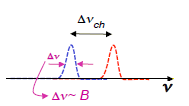
\includegraphics[scale=0.93]{ch3/image19}
	\captionof{figure}{ }
	\end{wrapfigure}
On défini alors l'efficacité spectrale  (à quel point la largeur spectrale est utilisée) comme le
rapport entre le débit et l'écart entre les canaux
\begin{equation}
{\eta _s} \buildrel \Delta \over = {B \mathord{\left/
 {\vphantom {B {\Delta {\nu _{ch}}}}} \right.
 \kern-\nulldelimiterspace} {\Delta {\nu _{ch}}}}
\end{equation}
On en tire
\begin{equation}
\Delta {\nu _d} > N.B/{\eta _s}{\rm{\approx }}N.\Delta {\nu _{FP}}/{\eta _s}
\end{equation}
Et donc
\begin{equation}
\frac{{\Delta {\nu _d}}}{{\Delta {\nu _{FP}}}} = {\cal F} > \frac{N}{{{\eta _s}}}
\end{equation}

\exemple{1. \textit{Si $R=99\%$ et $\eta_s=20$\%, quel est le nombre maximal de canaux ?}\\

On sait que $R$ impose la finesse (si pas de pertes, la finesse n'est liée qu'à $R$) qui vaut
à peu près $\mathcal{F}\approx 312$. Il faut donc que $312> N/\eta_s\ \Leftrightarrow\ 
N < 0.2*312 = 62$ canaux. C'est raisonnable, mais déjà un bon nombre.}\ \\

\exemple{2. \textit{Si $n=1$ (air entre les semi-miroirs) et $B=10$ Gbits/s, quelle est alors la longueur
de la cavité ?}\\
On sait que $\Delta\nu_{FP} = B$ et que $\Delta \nu_\lambda = c/(2dn) = \mathcal{F}$. Dès lors,
$\Delta_{FP}\approx FP \Rightarrow d = c/(2FB)=50\mu$m. Avec une cavité de cette taille, on pourra
sélectionné un seul des 62 canaux.}

\subsubsection{Tunability?}
	\begin{wrapfigure}[5]{l}{6.5cm}
	\vspace{-8mm}
	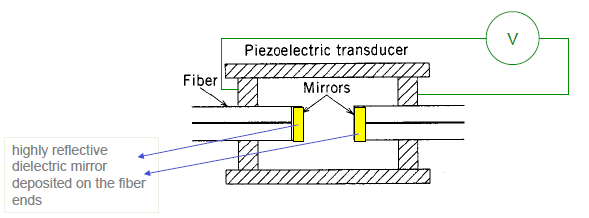
\includegraphics[scale=0.4]{ch3/image20}
	\captionof{figure}{ }
	\end{wrapfigure}
En pratique, comme $\Delta \nu_d = c/(2dn_{eff})$ on peut jouer sur $n_{eff}$ et $d_{eff}$
On peut modifier $d$ à l'aide d'une monture piézoélectrique et modifier $n$ à l'aide de 
cristaux liquides (dont $n$ change en fonction de la tension appliquée). \\

\subsection{Bragg grating filters}
On peut construire une cavité FP entre deux miroirs de Bragg. Ces-derniers jouent alors le rôle
des semi-miroirs. Le spectre en transmission dépend alors de la séparation entre les réseaux.
Le gap entre les réseau peut être vu comme un "défaut" qui crée un niveau d'énergie permis. 
L'énergie va alors se regrouper au centre pour avoir une transmission qui tend vers l'unité.

\newpage
\subsection{Multilayer dielectric thin-film filters (TFF)}
Il s'agit de la technologie la plus utilisée. En plaçant un dépot, en laissant une couche, puis
un nouveau dépot puis une espace plus important pour faire une cavité on crée la première partie
et on répète l'opération. A la fin, la structure créée sera de type Bragg-Cavité-Bragg. Comme les
réseaux de Bragg sont petits, il y a de fortes chances que l'onde évanescente d'une cavité 
atteigne l'autre : il y aura couplage entre les cavités.

\begin{center}
	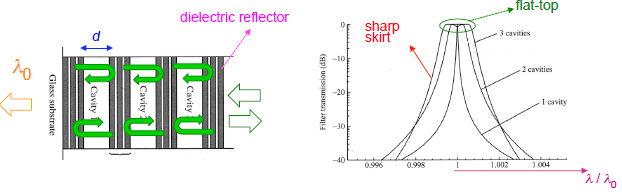
\includegraphics[scale=0.54]{ch3/image21}
	\captionof{figure}{ }
\end{center}

Il s'agit donc d'une cavité FP où les miroirs sont réalisés en utilisant des fines couches de
diélectriques. La bande passante du filtre sera fonction de l'épaisseur de la cavité $d$. La
fonction de transfert du filtre ressemble beaucoup à celle du PB mais avec un sommet beaucoup plus
plat et une décroissante des flancs bien plus rapide, d'ou l'intérêt de cette configuration.




\subsection{Acousto-optic tunable filters (AOTF)}
	\begin{wrapfigure}[9]{l}{8.5cm}
%	\vspace{-5mm}
	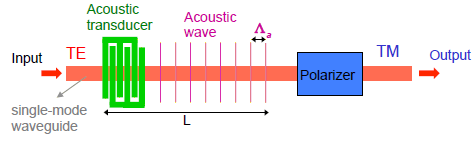
\includegraphics[scale=0.65]{ch3/image22}
	\captionof{figure}{ }
	\end{wrapfigure}
Le principe est que le signal d'entrée (mode $TE$) génère une onde acoustique dans la matériau. Cette onde acoustique va générer une modification de l'indice sous la forme d'un réseau via l'effet
élasto-optique. Ce réseau va coupler l'énergie d'une état de polarisation à un autre (vers le 
mode $TM$) à la longueur d'onde $\lambda_0$ qui satisfait la condition de Bragg
\begin{equation}
{k_{TM}} = {k_{TE}} \pm {K_a}\qquad\qquad\qquad
\frac{{{n_{TE}}}}{{{\lambda _0}}} = \frac{{{n_{TM}}}}{{{\lambda _0}}} \pm \frac{1}{{{\Lambda _a}}}
\end{equation}
On place alors un polariseur à la sortie orthogonal à la polarisation d'entrée ($TE$). Dès lors, 
seul le signal à $\lambda_0$ est transmis! Un exemple est donné au \textit{slide 36}.




\section{Multiplexers and Demultiplexers}
Les multiplexeur (MUX) et démultiplexeur (DEMUX) sont des composants importants dans chaque système
WDM. Le but d'un MUX est de combiner des signaux optiques de différentes longueur d'ondes venant de
fibres différentes et de les coupler en une seule fibre. Le DEMUX a la fonction inverse. 

\begin{center}
	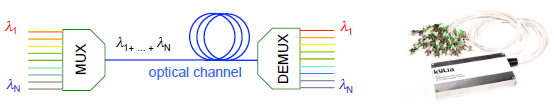
\includegraphics[scale=0.65]{ch3/image23}
	\captionof{figure}{ }
\end{center}

Le même dispositif peut être utilisé pour faire les deux, mais les performances des DEMUX ont des
critères plus stricts pour éviter le crosstalk. Il existe deux catégories de MUX/DEMUX : ceux 
basés sur les propriétés de diffraction et ceux basés sur les propriétés de la lumière 
(interférences).


\subsection{Grating-based Mux/Demux}
	\begin{wrapfigure}[9]{l}{8.5cm}
%	\vspace{-5mm}
	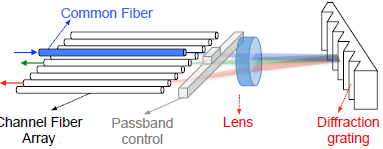
\includegraphics[scale=0.65]{ch3/image24}
	\captionof{figure}{ }
	\end{wrapfigure}
Le principe se base sur la loi des réseaux $\sin ({\theta _i}) - \sin ({\theta _r}) = 
m\frac{\lambda }{\Lambda }$.
La lumière arrive d'une fibre unique. A sa sortie, la lumière est collimatée en faisceau parallèles
à l'aide d'une lentille et celle-ci est incidente sur un réseau. Celui-ci diffracte la lumière et
sépare les composantes en longueur d'ondes qui repassent dans la lentille qui les "focus" dans
différentes fibres, dépendantes de la longueur d'onde. Attention aux pertes par dépendance de 
polarisation dans ces systèmes.


\subsection{Interference based Mux/Demux}
\subsubsection{1. Arrayed waveguide grating}
	\begin{wrapfigure}[11]{r}{8.5cm}
	\vspace{-5mm}
	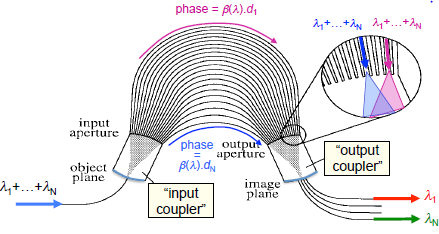
\includegraphics[scale=0.65]{ch3/image25}
	\captionof{figure}{ }
	\end{wrapfigure}
Il s'agit de la généralisation d'un interféromètre de Mach-Zehnder. On divise le signal en plus
de deux parties et on les recombine à la sortie après avoir accumulé des phases différentes. La 
longueur optique de chaque guide d'onde introduit une délai dépendant de la longueur d'onde à 
l'entrée du coupleur de sortie. Dans le coupleur, les faisceaux de tous les guides d'ondes interfèrent. Il en résulte un motif d'interférence dépendant de la longueur d'onde dans le "plan d'image" de sorte que chaque longueur d'onde soit couplée dans une fibre de sortie différente.
Pour les caractéristiques, voir le \textit{slide 39}.

\subsubsection{Fiber-Bragg gratings}
\begin{center}
	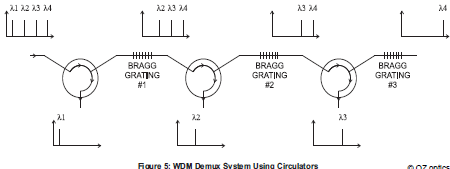
\includegraphics[scale=0.65]{ch3/image26}
	\captionof{figure}{Lorsqu'une image vaut mieux qu'un long discours}
\end{center}
\newpage
\subsubsection{3. Demux based on cascaded dielectric thin-film filters}
	\begin{wrapfigure}[7]{r}{6.5cm}
	\vspace{-5mm}
	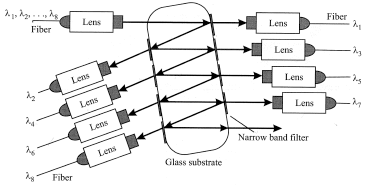
\includegraphics[scale=0.65]{ch3/image27}
	\captionof{figure}{ }
	\end{wrapfigure}
Le principe est de mettre en cascade un certain nombre de film filtres fin : chacun laisse passer
une longueur d'onde différente et réfléchi toute les autres. L'avantage est de former un dispositif
très compact qui ne dépend quasi pas de la température (avantage par rapport à Bragg qui se 
dilate). Les caractéristiques sont données au \textit{slide 41.}\\

\section{Optical add-drop multiplexers (OADM)}
	\begin{wrapfigure}[12]{l}{8.5cm}
%	\vspace{-5mm}
	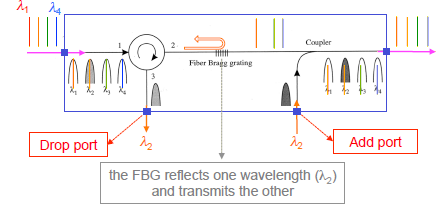
\includegraphics[scale=0.7]{ch3/image28}
	\captionof{figure}{ }
	\end{wrapfigure}
Le rôle principal d'un OADM est de supprimer une longueur d'onde particulière d'une groupe de
longueur d'onde (\textit{drop}) ou en ajouter une particulière (\textit{add}) tout en maintenant
l'intégrité du signal pour toutes les autres longueurs d'onde (canaux). On les utilise typiquement
pour des réseau comme celui de Belnet. En venant d'Anvers, on sortira l'information pour Bruxelles
mais celle de Namur ira tout droit. On peut voir ça comme des connecteurs modulables. 





















